\subsection{Part 1}
The common-drain amplifier shown in Figure 1 was constructed, using 2 $10k$ \si{\ohm} resistors in parallel for the $5k$ \si{\ohm} resistor.
These resistors were measured to have a parallel resistance of $4.924k$\si{\ohm}.

\FloatBarrier

\begin{figure}[h!]
	\centering
	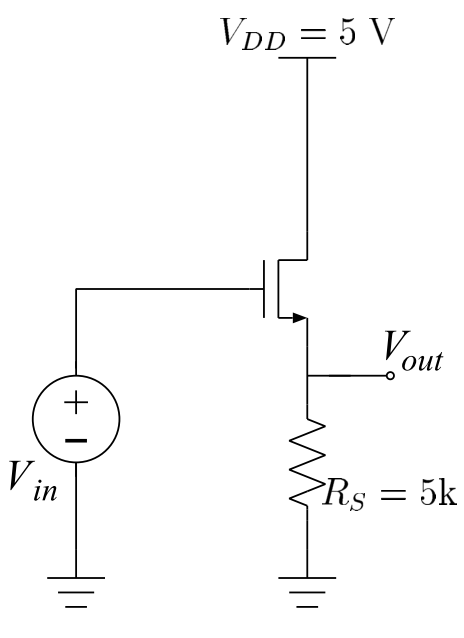
\includegraphics[scale=0.75]{./images/circuit_1.PNG}
	\caption{Circuit 1}
	\label{fig:circuit_1}
\end{figure}

\FloatBarrier

With $V_{DS}$ constant at $5$\si{\volt}, $V_{GS}$ was swept from 0 to $5$\si{\volt} to obtain the voltage transfer characteristic shown in Figure 2 and Table 1.

\FloatBarrier

\begin{figure}[h!]
	\centering
	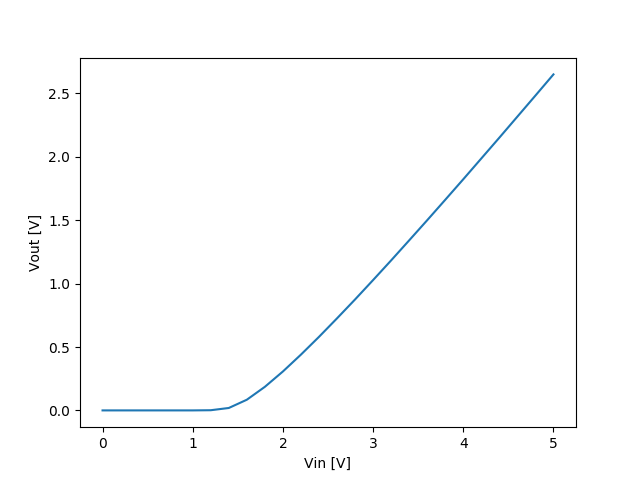
\includegraphics[scale=0.75]{./images/part1_vtc.PNG}
	\caption{Vout vs Vin for the common-drain amplifier}
	\label{fig:part1_vtc}
\end{figure}

\FloatBarrier

\begin{table}[h!]
	\centering
	\caption{Figure (\ref{fig:part1_vtc}) Data}
	\label{tab:part1_vtc}
	\csvautotabular{./tables/part1_vtc.csv}
\end{table}

\FloatBarrier

For this circuit, Vout = $I_{D}$ $R_{S}$, so Vout will be zero while the transistor is in cutoff. Afterwards, even when Vin = $5$\si{\volt}, $V_{DS}$ is more than Vin - $V_{t}$ so that the transistor is in saturation any time it is on.
The threshold voltage appears to be around $1.4$\si{\volt}.
For maximum possible input swing, we biased the circuit at $V_{GS}$ = $3.3$\si{\volt}.

Next, we applied a $10$\si{\milli\volt} signal to Vin, starting off at $1$\si{\kilo\hertz} under the assumption that the amplifier will perform better when at lower frequencies.
We subsequently increased the frequency to $100$\si{\kilo\hertz} and $1$\si{\mega\hertz}. Oscilloscope screenshots are shown for each frequency in Figures 3, 4, and 5, respectively.
The gains at each frequency are tabulated in Table 2.


\FloatBarrier

\begin{figure}[h!]
	\centering
	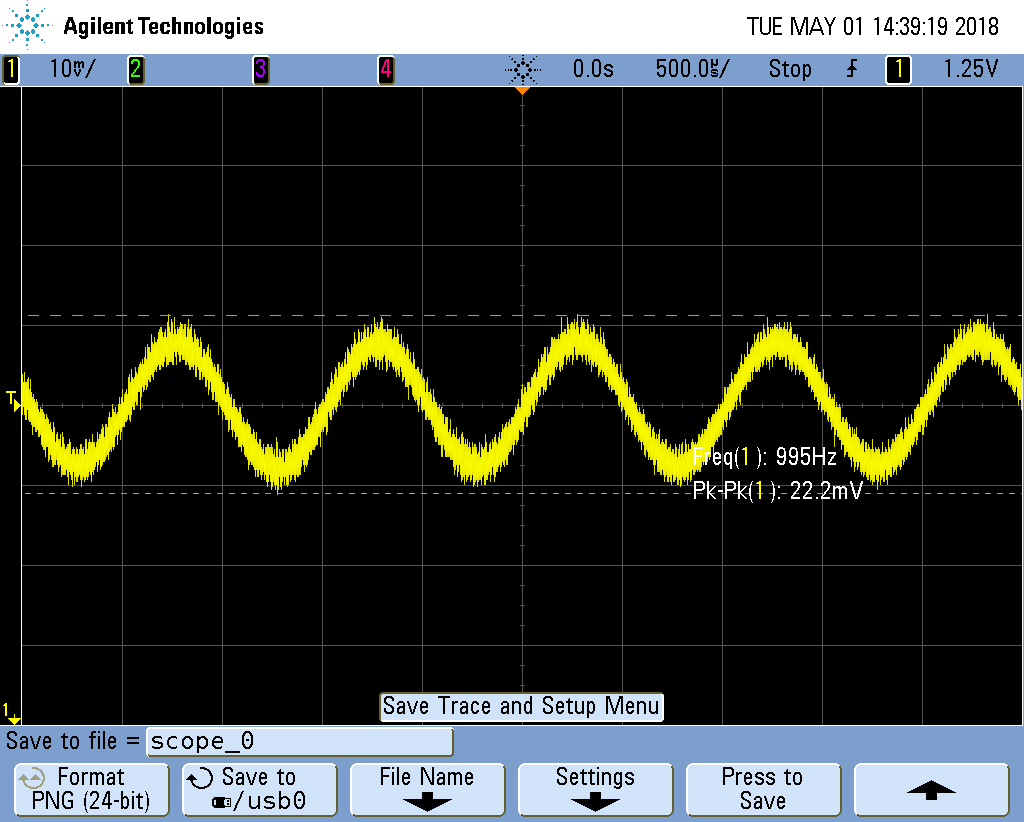
\includegraphics[scale=0.75]{./images/SCOPE_0.PNG}
	\caption{Amplified waveform of a $1$\si{\kilo\hertz} signal of peak-to-peak amplitude of $20$\si{\milli\volt}}
	\label{fig:SCOPE_0}
\end{figure}

\FloatBarrier

\begin{figure}[h!]
	\centering
	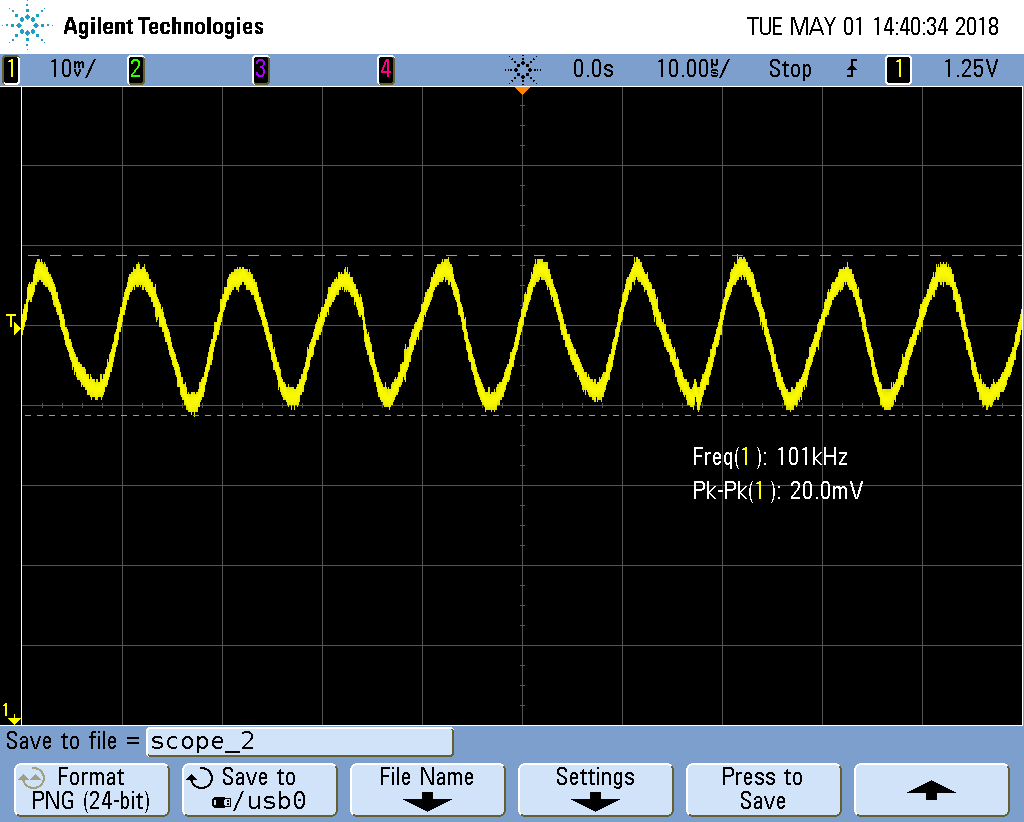
\includegraphics[scale=0.75]{./images/SCOPE_2.PNG}
	\caption{Amplified waveform of a $100$\si{\kilo\hertz} signal of peak-to-peak amplitude of $20$\si{\milli\volt}}
	\label{fig:SCOPE_2}
\end{figure}

\FloatBarrier

\begin{figure}[h!]
	\centering
	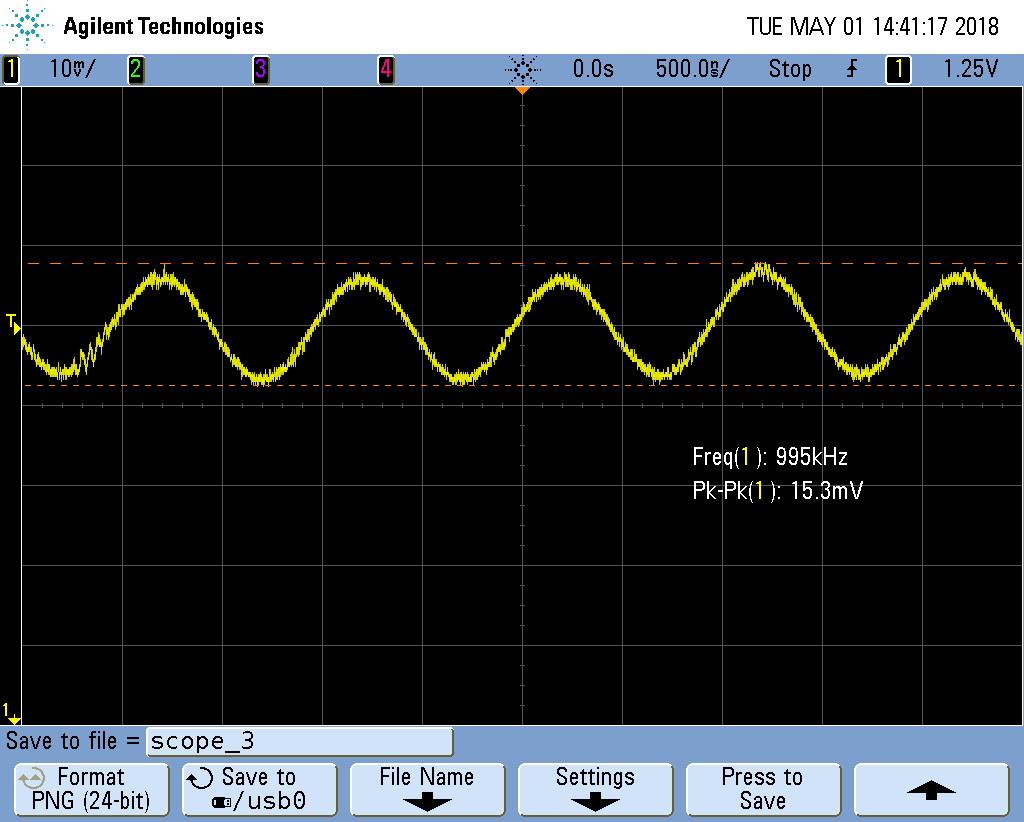
\includegraphics[scale=0.75]{./images/SCOPE_3.PNG}
	\caption{Amplified waveform of a $1$\si{\mega\hertz} signal of peak-to-peak amplitude of $20$\si{\milli\volt}}
	\label{fig:SCOPE_3}
\end{figure}

\FloatBarrier

\begin{table}[h!]
	\centering
	\caption{Figure (\ref{fig:SCOPE_3}) Data}
	\label{tab:gain_part1}
	\csvautotabular{./tables/gain_part1.csv}
\end{table}

\FloatBarrier

The varying gains as a function of frequency shows that the amplifier is not as effective at higher frequencies. In order for this circuit to function as a voltage follower or buffer as it was intended, the signal frequency should stay near $100$\si{\kilo\hertz}.

This procedure was repeated when biasing the transistor $10$\si{\milli\volt} higher. Results are shown in Figures 6, 7, and 8, respectively, and gains are tabulated in Table 3.

\FloatBarrier

\begin{figure}[h!]
	\centering
	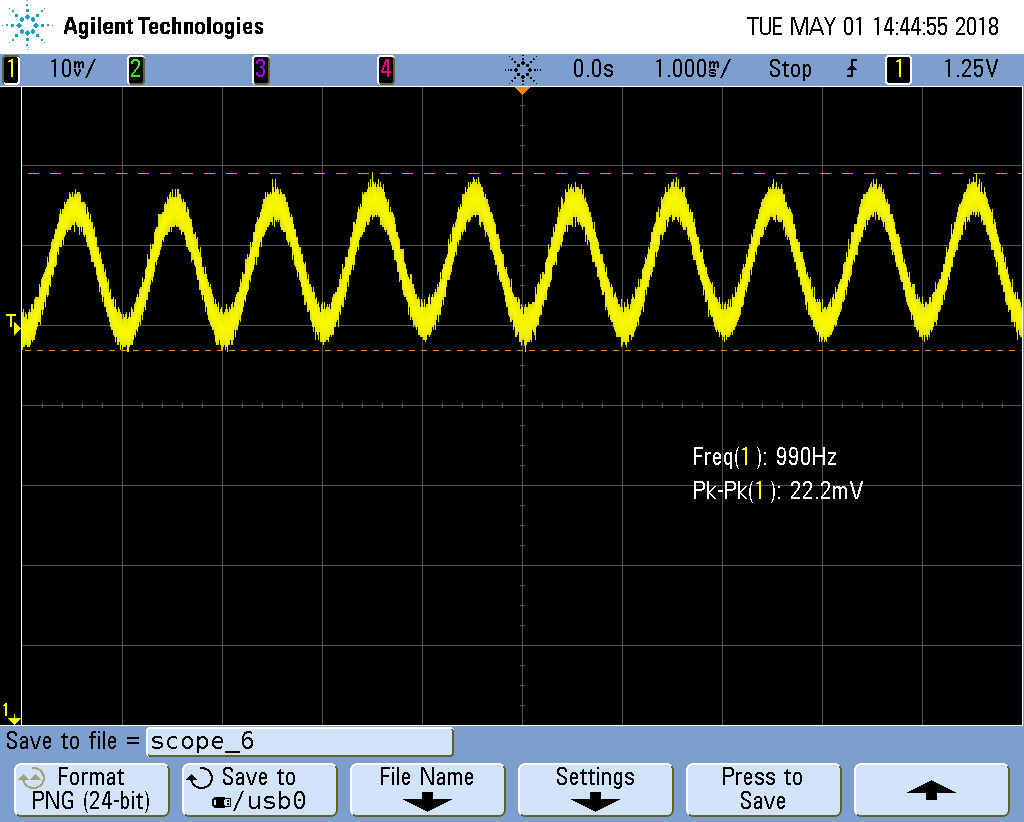
\includegraphics[scale=0.75]{./images/SCOPE_6.PNG}
	\caption{Amplified waveform of a $1$\si{\kilo\hertz} signal of peak-to-peak amplitude of $20$\si{\milli\volt}}
	\label{fig:SCOPE_6}
\end{figure}

\FloatBarrier

\begin{figure}[h!]
	\centering
	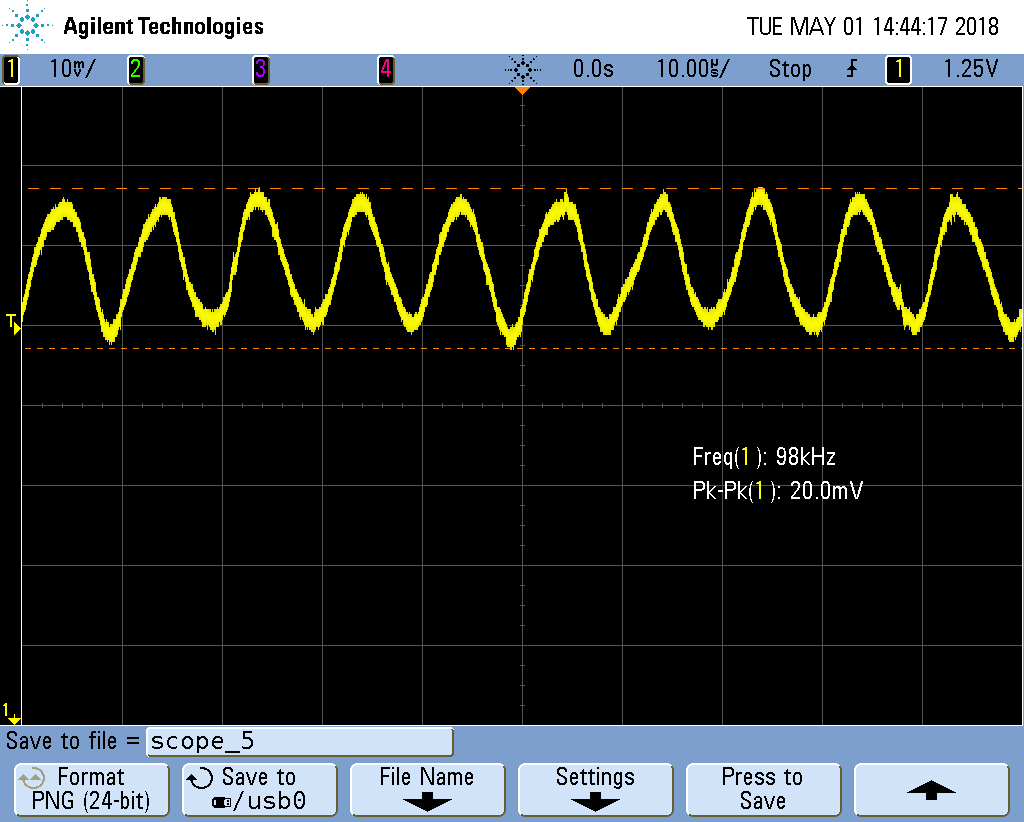
\includegraphics[scale=0.75]{./images/SCOPE_5.PNG}
	\caption{Amplified waveform of a $100$\si{\kilo\hertz} signal of peak-to-peak amplitude of $20$\si{\milli\volt}}
	\label{fig:SCOPE_5}
\end{figure}

\FloatBarrier

\begin{figure}[h!]
	\centering
	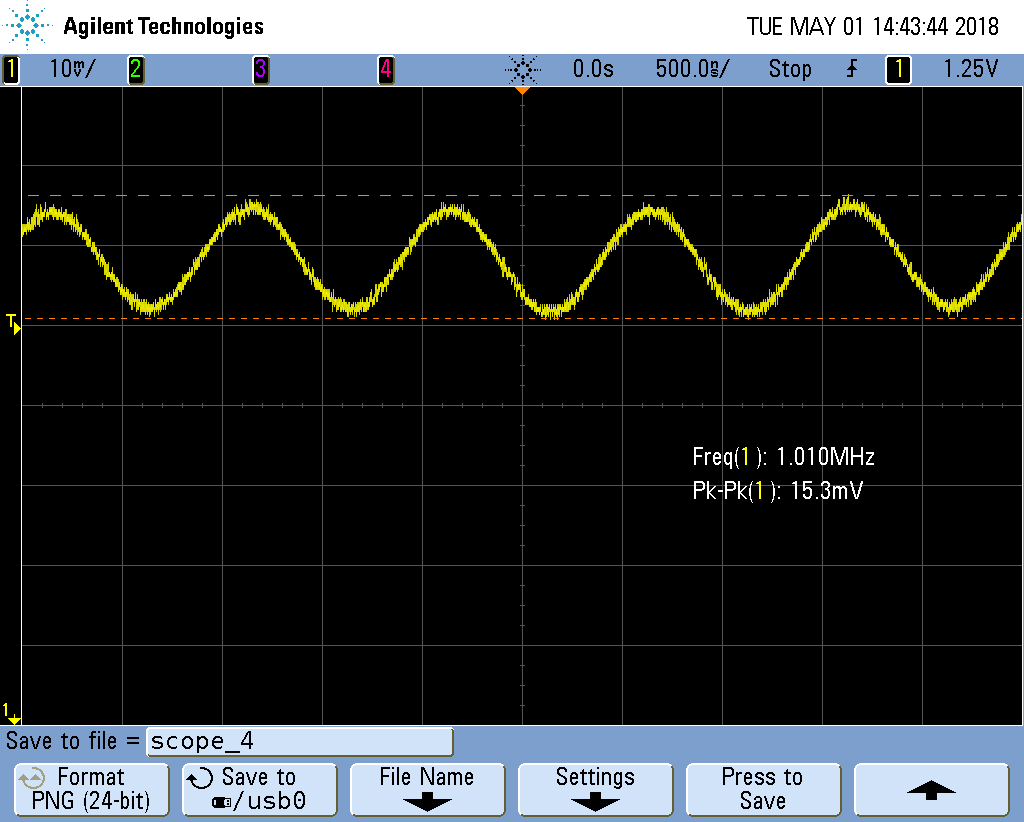
\includegraphics[scale=0.75]{./images/SCOPE_4.PNG}
	\caption{Amplified waveform of a $1$\si{\mega\hertz} signal of peak-to-peak amplitude of $20$\si{\milli\volt}}
	\label{fig:SCOPE_4}
\end{figure}

\FloatBarrier

\begin{table}[h!]
	\centering
	\caption{Figure (\ref{fig:SCOPE_4}) Data}
	\label{tab:gain_part1_plus10mV}
	\csvautotabular{./tables/gain_part1_plus10mV.csv}
\end{table}

\FloatBarrier

Due to the nearly uniform slope of the VTC in the saturation region, the gain as a function of bias is nearly constant. Thus, these waveforms and gains are practically identical to what was seen earlier.
